% This is samplepaper.tex, a sample chapter demonstrating the
% LLNCS macro package for Springer Computer Science proceedings;
% Version 2.20 of 2017/10/04
%
\documentclass[runningheads]{llncs}
%
\usepackage{graphicx}
% Used for displaying a sample figure. If possible, figure files should
% be included in EPS format.
%
% If you use the hyperref package, please uncomment the following line
% to display URLs in blue roman font according to Springer's eBook style:
% \renewcommand\UrlFont{\color{blue}\rmfamily}
\usepackage{amsmath,amssymb}
\usepackage{amsfonts}
\usepackage{subfigure}

\begin{document}
%
\title{Deep Triplet Network adopting the Kernel and the Range Space Learning for Wi-Fi Handwritten Signature Verification}
%
\titlerunning{Triplet Network adopting KAR Learning for Wi-Fi Signature Verification}
% If the paper title is too long for the running head, you can set
% an abbreviated paper title here
%
\author{Young-Woong Kwon \and Jooyoung Kim \and Kar-Ann Toh}
%
\authorrunning{Y. Kwon et al.}
% First names are abbreviated in the running head.
% If there are more than two authors, 'et al.' is used.
%
\institute{
School of Electrical and Electronic Engineering, Yonsei University, 50 Yonsei-ro, Seodaemun-gu, Seoul 03722, Republic of Korea\\
\email{\{herokwon, harrykim, katoh\}@yonsei.ac.kr}}
%
\maketitle              % typeset the header of the contribution
%
\begin{abstract}
%The abstract should briefly summarize the contents of the paper in 15--250 words.
In this paper, we propose a system for identity verification based on the handwritten signature signals captured by the Wi-Fi CSI signals. 
The kernel and the range space learning is initially adopted for refining the triplet inputs for fast loss convergence by mining the distinctive inputs from the training Wi-Fi signature signals. 
Subsequently, the triplet network utilizing the ConvNet structure is trained with the mined triplet inputs based on L-2 distance comparison. 
Our experiments on an in-house Wi-Fi handwritten signature signal dataset show encouraging verification accuracy with faster training loss convergence comparing with the baseline triplet network and the Siamese network.

\keywords{Wi-Fi signature signal \and in-air handwritten signature verification \and the Kernel and the Range space projection learning \and triplet network}
\end{abstract}
%
%
%
\section{Introduction}

In recent years, several behavioral biometric traits for identity authentication have been investigated in view of their rigid physical body independence~\cite{bailador2011analysis}. Among the behavioral biometrics, the signature-based user authentication~\cite{sanmorino2012survey,galbally2015line} is attracting considerable interest with the development of in-air signature recognition systems~\cite{jeon2012system,sesa2012information,malik20183dairsig}.
With the help of sensors such as the depth camera~\cite{malik20183dairsig} or mobile sensor~\cite{jeon2012system}, the in-air signature recognition system has lower spatial constraint in the signature acquisition process than the contact-based authentication systems. 

Recently, the commercial Wi-Fi device has been adopted for in-air signature authentication due to its easy accessible property \cite{moon2017air}. Based on the distortion of the  Wi-Fi CSI signal according to the user's gestures, the in-air signature recognition system showed reasonable user verification performance~\cite{moon2017air}. 
% omitted
%However, the previous works on Wi-Fi signal based user authentication systems~\cite{hong2016wfid,moon2017air} utilized the conventional feature extraction method such as the Principal Component Analysis. Since the conventional feature extraction method is not enough to extract the direction- or pose-invariant features from the acquired in-air data, 
More recently, some studies attempted to implement the deep learning algorithms in Wi-Fi signal-based user authentication systems to improve the verification performance ~\cite{shi2017smart,pokkunuru2018neuralwave}. 

In this paper, we utilize the deep triplet network for identity verification based on the Wi-Fi CSI signature signal. To achieve not only the desired verification accuracy but also a fast training speed, we adopt the kernel and the range (KAR) space leaning~\cite{toh100,toh2018learning,toh2018analytic,toh2018gradient} in order to mine the distinctive triplet inputs. Subsequently, the triplet network utilizing the ConvNet structure as a feature extractor is trained based on the L-2 distance comparison.

The main contributions of our work can be summarized as follows:
\begin{itemize}
\item Proposal of a system for identity verification based on the Wi-Fi handwritten signature signals using a deep triplet network.
\item Adopted the kernel and the range (KAR) space learning in order to mine the distinctive triplet inputs which boost the convergence speed of the training loss in triplet network.
\item Provision of the experimental study on an in-house Wi-Fi handwritten signature signal dataset collected from 50 subjects.
\end{itemize}

The paper is organized as follows: related works including the triplet network and KAR space learning will be introduced in Section 2 for immediate reference. Our proposed method will be discussed in Section 3. Section 4 describes our experimental results and analysis. Some concluding remarks will be given in Section 5.


\section{Related works}

\subsection{Triplet network}
% triplet network
The triplet network is considered a metric learning based model~\cite{weinberger2006distance} which aims to learn useful representations by means of distance comparison~\cite{hoffer2015deep}. 
\textbf{It is often seen in person re-identification~
\cite{chen2017beyond,cheng2016person,ding2015deep,schroff2015facenet,wang2016joint}. Re-identification is an identification problem using the images/videos taken from a different camera~\cite{bedagkar2014survey}. The individual identities are matched based on identity discriminative features. In these problems, the distinction among the classes is challenging since the features are relatively weak compared to the background features. To address this problem, the triplet network optimizes the embedding training data space such that data points with the same identity are closer to each other than those with different identities~\cite{hermans2017defense}.}

\textbf{The triplet network receives triplet pairs as its input which is made from a combination of the input data. Since not all triplet samples are contribute to the training ~\cite{schroff2015facenet}, recent issues have highlighted which input pairs will be used for training. To optimize the training process by utilizing only some part of the triplet pairs, \cite{cheng2016person,ding2015deep,wang2016joint} generated triplet only from limited classes, which are randomly selected in each iteration.}

\textbf{Recently, \cite{schroff2015facenet} adopted additional triplet mining process for the faster convergence speed. They utilized large mini-batch at each training iteration and selected the triplet based on the training network rather than the random sampling. However, this strategy needed a few thousand exemplars of mini-batch in every training iteration to select the triplet pairs which burden the time.}

%the triplet network receives triplet data as an input, which consists of the anchor, positive and negative data. The objective function of the triplet network is to place the feature vectors in the appropriate separation space by putting the positive (similar) data closer to the anchor (reference) data and keeping the negative (dissimilar) data away from the anchor data.
%.... (1. tell how the triplet network solves the problem and not unrelated parts of it. 2. Tell what further issues arise from triplet network?)

% optimize training
%Not clear and no link to above, rewrite this sentence.
%Since myriad combinations of the triplet pairs can be generated in the training set, training with all possible triplets is time-consuming and unnecessary. To optimize the training process by utilizing only some part of the triplet pairs, \cite{cheng2016person,ding2015deep,wang2016joint} generated triplet only from limited classes, which are randomly selected in each iteration.
%Recently, \cite{schroff2015facenet} adopted triplet mining strategy for the faster convergence speed. They utilized large mini-batch at each training iteration and selected the triplet based on the training network.
%However, they needed a few thousand exemplars of mini-batch in every training iteration to select the triplet pairs.

% Rel works: KAR learning
\subsection{Kernel and the range space learning}\label{kar}

The multilayer feedforward neural networks is generally trained by the gradient descent method based on backpropagation \cite{goodfellow2016deep}.
However, setting the learning parameters such as learning rate or momentum value is time consuming and yet important to arrive at reasonable solution.

Recently, a gradient-free learning framework based on the kernel and the range (KAR) space manipulation has been developed for multilayer network learning~\cite{toh2018learning,toh2018gradient}.
The learning method is grounded on linear algebra with neither learning parameters nor iteration are needed in training.

% Karnet structure and mining samples.
Let the training dataset $\mathbf{X}\in{\mathbb{R}}^{m \times (n+1)}$ and $\mathbf{G}\in{\mathbb{R}}^{m \times n}$ as the network outputs.
Then the multilayer neural network structure can be written in linear equation form as follows:
\begin{equation}
    \mathbf{G} = \sigma\left(\left[\mathbf{1},\sigma\left(\dots\left[\mathbf{1},\sigma\left(\left[\mathbf{1},\sigma\left(\mathbf{X}\mathbf{W}_{1}\right)\right]\mathbf{W}_{2}\right)\right]\dots\mathbf{W}_{(i-1)}\right)\right]\mathbf{W}_{i}\right),
\end{equation}
where $\mathbf{W}_{1}\in{\mathbb{R}}^{(n+1) \times h_{1}}$,$\mathbf{W}_{2}\in{\mathbb{R}}^{(h_{1}+1) \times h_{2}}$,$\dots,\mathbf{W}_{i}\in{\mathbb{R}}^{(h_{(i-1)}+1) \times n}$,$\mathbf{1}=\left[1,\dots,1\right]^{T}\\
\in{\mathbb{R}}^{m \times 1}$ and $\sigma(.)$ is activation function.
By adopting the one-hot encoded target $\mathbf{Y}\in{\mathbb{R}}^{m \times n}$ instead of network output $\mathbf{G}$, The trained weight matrices $\mathbf{W}_{i}$ using KAR space manipulation can be obtained as follows~\cite{toh2018gradient}:

\begin{equation}
    \mathbf{W}_{i} = \left[\mathbf{1},\sigma\left(\dots\left[\mathbf{1},\sigma\left(\left[\mathbf{1},\sigma\left(\mathbf{X}\mathbf{W}_{1}\right)\right]\mathbf{W}_{2}\right)\right]\dots\mathbf{W}_{(i-1)}\right)\right]^{\dagger}\sigma^{-1}\left(\mathbf{Y}\right).
\end{equation}



%% Methods
\section{Proposed System}

% Methods: System overview(Fig.1)
In this section, we propose an identity verification system based on the Wi-Fi based in-air handwritten signature (which will be called Wi-Fi signature signals hereafter) using the triplet network~\cite{hoffer2015deep}. Fig.1 shows an overview of the proposed system utilizing the kernel and the range (KAR) space learning~\cite{toh2018learning,toh2018gradient} for the triplet mining and the triplet network.
Essentially, the KAR space projection learning is trained and utilized to generate the triplet input data by mining the hard positive and the hard negative samples from each given anchor sample in the training dataset (see item (a) in Fig.~\ref{fig1}).
Subsequently, the ConvNet structure in the triplet network (see item (b) in Fig.~\ref{fig1}) is trained with the mined triplet data based on the triplet loss function using L-2 distance comparison (see item (c) in Fig.~\ref{fig1}).
The following subsections describe the details of the triplet mining using KAR space learning and the triplet network.

% Figure 1
\begin{figure}[!ht]
    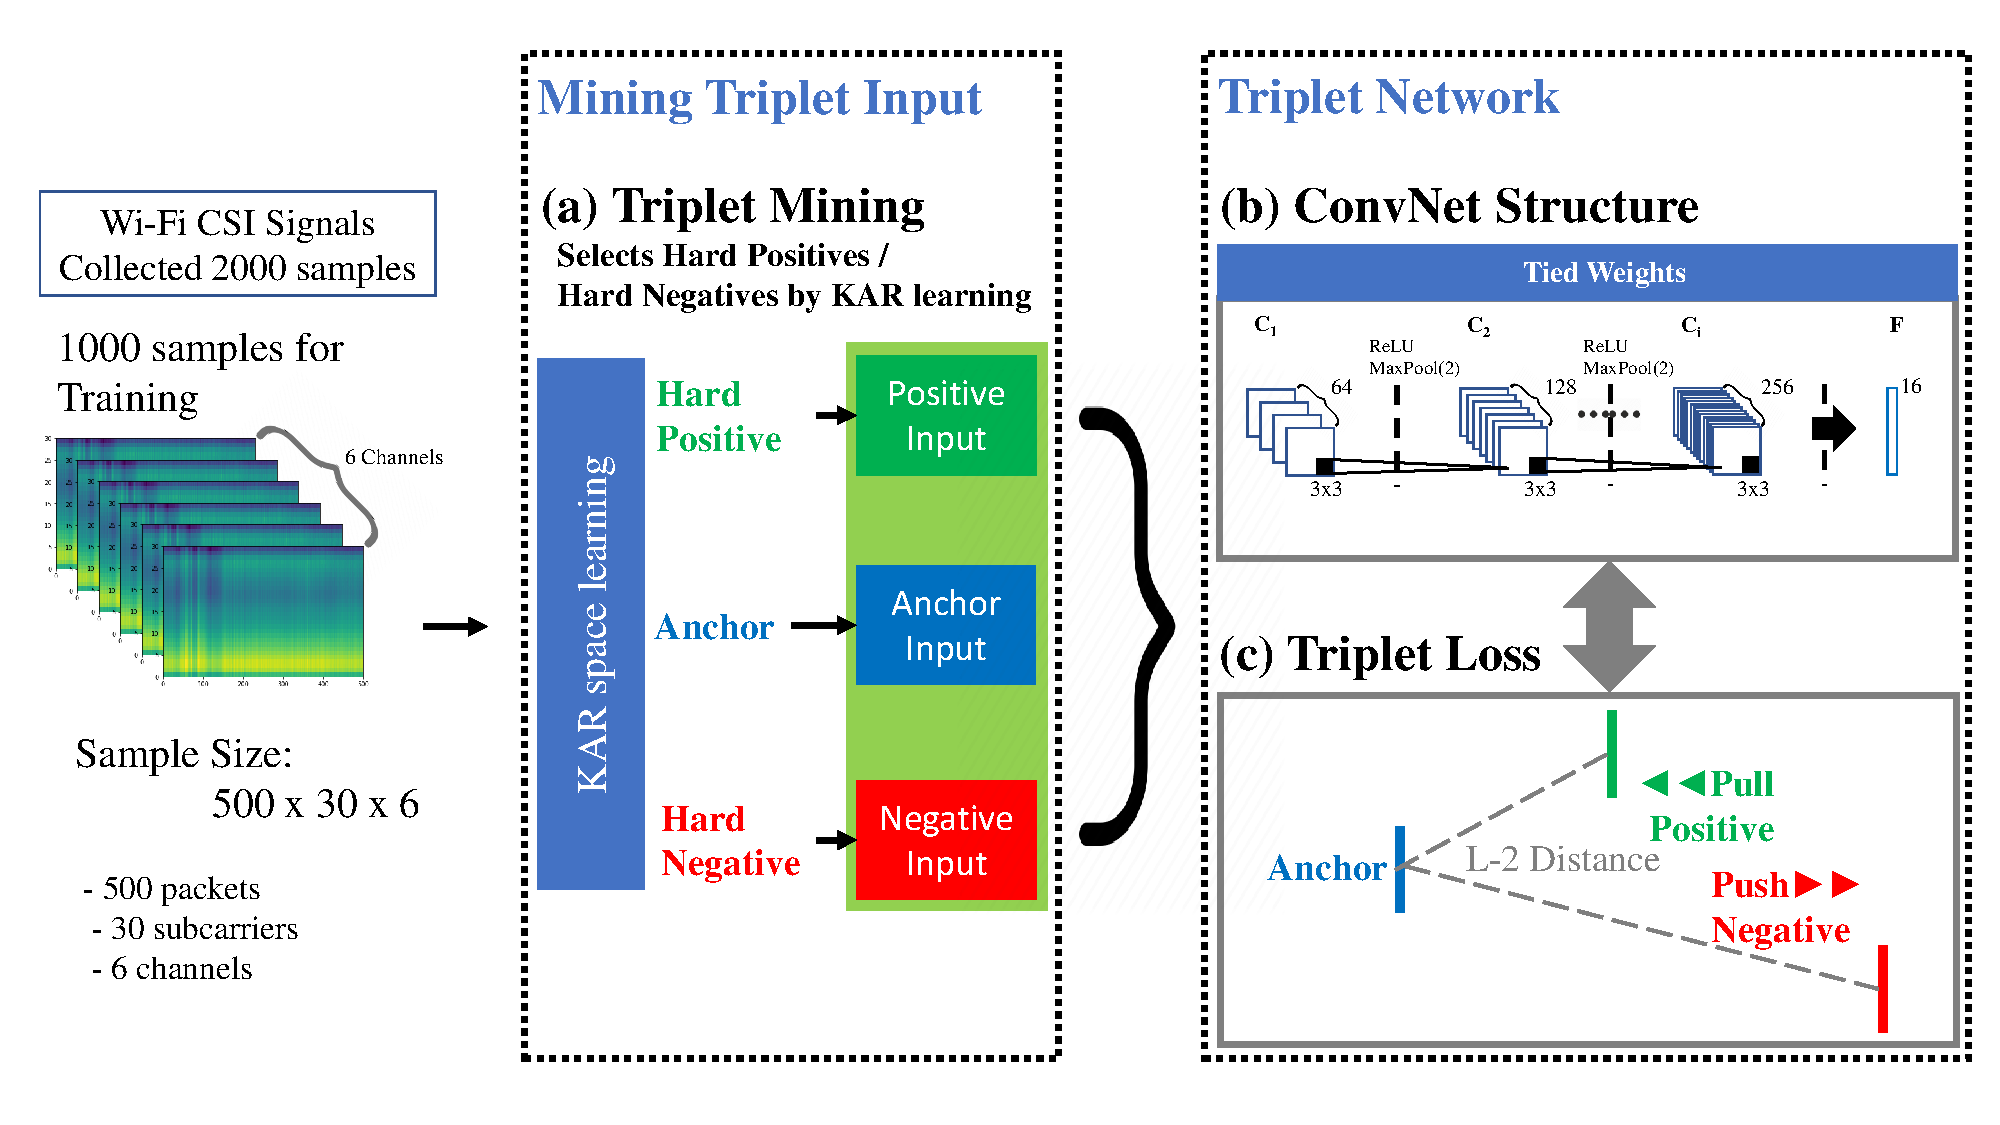
\includegraphics[width=\textwidth]{fig1_tcnn_kar_v5}
    \caption{An overview of the proposed system.} \label{fig1}
\end{figure}

% Methods: KAR learning
\subsection{Triplet mining using kernel and the range space learning}
%1. Need to explain what is "hard" first.
%2. Also, need to explain "anchor sample" before using it.
% description of anchor sample
% loss convergence problem
% we need hard sample selection

\textbf{The triplet network receives triplet data as an input, which consists of the reference data (will be called anchor hereafter) and corresponding positive (same class with the anchor) and negative data (different class with the anchor). The objective function of the triplet network is to place the feature vectors in the appropriate separation space by putting the positive data closer to the anchor data and keeping the negative data away from the anchor data.}

According to \cite{schroff2015facenet}, it is important to select the hard positive and the hard negative samples from each given anchor sample for faster loss convergence when training the triplet network.
The hard positive sample denotes the positive sample whose distance to the anchor sample is the greater than others (which is most likely to be misclassified as a negative sample) while the hard negative sample denotes the negative sample whose distance to the anchor sample is the smaller (which is most likely to be misclassified as a positive sample). However, there is no information about which sample is hard positive or negative before we train the network.

In this work, we propose to adopt the kernel and the range (KAR) space learning (see Section~\ref{kar} for details) as a pretraining network to mine the hard positive/negative samples from the given anchor sample. Since the KAR space learning has no iterative learning process, we can mine the triplet samples without using the time consuming backpropagation training process.
 
By training the network with using the single shot KAR space learning method, we can calculate the L-2 distance between every training samples by using the output vector from the KAR space network. Taking each training sample as an anchor sample $\mathbf{x}_{anc}$, to measure the distance between $\mathbf{x}_{anc}$ and other samples, the trained network output given by:

\begin{equation}
    f\left(\mathbf{X}\right) = \sigma\left(\left[\mathbf{1},\sigma\left(\dots\left[\mathbf{1},\sigma\left(\left[\mathbf{1},\sigma\left(\mathbf{X}\cdot\mathbf{W}_{1}\right)\right]\mathbf{W}_{2}\right)\right]\dots\mathbf{W}_{(i-1)}\right)\right]\mathbf{W}_{i}\right),
\end{equation}

is used to generate the hard positive and hard negative samples.
The hard positive sample $\mathbf{x}_{pos}$ and the hard negative sample $\mathbf{x}_{neg}$ with respect to the anchor sample $\mathbf{x}_{anc}$ can be respectively to determined by:

\begin{equation}
    {\left\| {{f\left(\mathbf{x}_{anc}\right)} - {f\left(\mathbf{x}_{pos}\right)}} \right\|_2^2} \geq \mathrm{t}_{pos}, \label{pos}
\end{equation}
\begin{equation}
    {\left\| {{f\left(\mathbf{x}_{anc}\right)} - {f\left(\mathbf{x}_{neg}\right)}} \right\|_2^2} \leq \mathrm{t}_{neg},\label{neg}
\end{equation}

where $\mathrm{t}_{pos}$ and $\mathrm{t}_{neg}$ denotes the thresholds which determines whether a sample is hard positive/negative. Here we utilized equations~\eqref{pos} and~\eqref{neg} to select the hard positive/negative samples instead of just using the hardest positive/negative samples since the hardest samples are likely to be outliers which degrade the training process of the triplet network.
We empirically set the $\mathrm{t}_{pos}$ to 75 percentile of L-2 distance and $\mathrm{t}_{neg}$ to 25 percentile of L-2 distance and the final $\mathbf{x}_{pos}$ and $\mathbf{x}_{neg}$ are randomly selected among the samples which match the equations.

% Methods: ConvNets
\subsection{ConvNet structures}

To design the triplet network, we first need to select the feature extractor which converts the input triplet data into feature vectors. In this work, we utilize the ConvNet structure~\cite{lecun1998gradient} as a feature extractor since the three-dimensional data format of our preprocessed input signal can be regarded as an image data format with multiple channels. 

Our ConvNet structure (item (b) in Fig~\ref{fig1}) for the network consists of $i$ convolutional layers $\mathbf{C}_{i}$ and one fully-connected layer $\mathbf{F}$. The number of convolutional filters to be trained in each layer is empirically chosen as $\{64, 128, ...,  2^{6+i}\}$, with fixed filter size of $3\times3$ and stride of 1. The Rectified Linear (ReLU) function as an activation function and the Max-pooling layer are applied between each convolutional layer. Subsequently, the features from the last convolutional layer are directly flattened into a vector before the fully-connected layer $\mathbf{F}$.
The output vectors from the fully-connected layer are finally transformed using the sigmoid function following with the L-2 normalization.

%Since the networks utilize three ConvNet structures which ties the weights each other, noting here that three structures described in Fig~\ref{fig1} (b) are actually the same model.

% Methods: Triplet loss
\subsection{Triplet loss}

The triplet loss function was first seen in \cite{hoffer2015deep} to train the triplet network.
For the $i_{th}$ anchor input sample $\mathbf{x}_{anc,i}$, the triplet input is generated by grouping the hard positive input samples $\mathbf{x}_{pos,i}$ and the hard negative input samples $\mathbf{x}_{neg,i}$ selected based on the KAR space learning. The generated triplet input $\left\{\mathbf{x}_{anc,i},\mathbf{x}_{pos,i},\mathbf{x}_{neg,i}\right\}$ is then respectively transformed to the anchor, the positive and the negative feature vectors $\left\{\mathbf{v}_{anc,i},\mathbf{v}_{pos,i},\mathbf{v}_{neg,i}\right\}$ with the ConvNet structure.

Here, the triplet loss function is calculated by comparing the positive distance (L-2 distance between the anchor vector and the positive vector) and the negative distance (L-2 distance between the anchor vector and the negative vector) as follows:

\begin{equation}
    loss = \sum_i^N max\left({ \left[ {\left\| {{\mathbf{v}_{anc,i}} - {\mathbf{v}_{pos,i}}} \right\|_2^2} - {\left\| {{\mathbf{v}_{anc,i}} - {\mathbf{v}_{neg,i}}} \right\|_2^2}  + \alpha \right]}, 0 \right),\label{triplet}
\end{equation} 

where $N$ denotes the size of the mini-batch, ${\left\| . \right\|_2^2}$ denotes the L-2 distance and $\alpha$ denotes the preset margin.
The ConvNet structure using equation~\eqref{triplet} is thus trained to maximize the gap between the positive distance and the negative distance which should be larger than the margin $\alpha$.

\section{Experiments}

% Dataset
\subsection{Dataset}
 In order to evaluate the verification performance of the proposed system, the Wi-Fi CSI signature dataset \cite{moon2017air} with single position was utilized in our experiments. After adopting the data preprocessing process proposed in \cite{moon2017air}, the Wi-Fi CSI signature dataset consists of 2000 Wi-Fi CSI signature signals (4 directions $\times$ 10 samples $\times$ 50 identities) with the sample size of 500$\times$30$\times$6. We utilized only the absolute value from each complex CSI signal in our experiments since the 2.4Ghz Wi-Fi CSI signals have issues of device firmware in their phase signal~\cite{wang2015understanding}.

\subsection{Experimental settings}

\subsubsection{Performance evaluation}
The proposed system is evaluated under two cases: i) case I on comparison between the proposed system and other linear or deep learning-based methods based on verification accuracy, and case II on detailed comparison between the proposed system and the deep learning-based methods using receiver operating characteristic (ROC) curve and training loss curve. For the Case I, existing linear methods such as the least squares error estimation (LSE), the principal components analysis (PCA) [22] with LSE, the support vector machine (SVM) with different kernel function and total error rate minimization which adopts the reduced multivariate polynomial model as basis function (TER-RM2) \cite{toh2003fingerprint,toh2008between}, the deep learning-based Siamese network \cite{koch2015siamese} and the baseline triplet network \cite{hoffer2015deep} are included for performance benchmarking. The Siamese network and the baseline triplet network utilized the same ConvNet structures with the proposed system and only differed in their input data style and loss function.

The verification performance of the proposed system and other methods were evaluated in terms of Equal Error Rates (EER, \%) averaged from five runs of two-fold cross-validation test. Due to the memory constraint caused by the large data size, noting here that the deep learning-based methods utilized randomly sampled 9,500 negative pairs in the validation stage, which is the same number as the number of the positive pairs.

\subsubsection{Network Structure and Parameter Settings}
The multilayer feedforward network structure of KAR space learning is specified in Table~\ref{tab2}. With input data, size of 500$\times$30$\times$6, we set two network layers where the size of the each layer is 1024 and 16, respectively. Each layer is initialized with uniform distribution over [0, 1). We used $\sigma = {tan}^{-1}$ as an activation function following \cite{toh2018analytic}.

\begin{table}[]
    \caption{The network structure of the KAR space learning.}\label{tab2}
    \centering
    \begin{tabular}{|l|l|l|}
    \hline
    Layer   & Size     & Activation \\ \hline
    Input   & 500$\times$30$\times$6 &            \\
    Fully-Connected 1 & 1$\times$1$\times$1024 & $\sigma = {tan}^{-1}$     \\
    Fully-Connected 2 & 1$\times$1$\times$16  & $\sigma = {tan}^{-1}$     \\
    Output  & 1$\times$1$\times$50   &            \\ \hline
    \end{tabular}
\end{table}

For the proposed system and the deep learning-based methods, we utilized the same ConvNet structure as specified in Table~\ref{tab1}. We trained the network starting with a learning rate of 0.00005 and a mini-batch, size of 32. We optimized the loss by the Adam optimizer with L-2 penalty of 0.0002 except for the output layer. The output layer is regularized with L-2 penalty of 0.0001. We initialized all network weights in the convolutional layers with normal distribution of zero-mean and standard deviation of 0.01. Biases were also initialized with normal distribution of 0.5 mean and standard deviation of 0.01. For the triplet networks, the hyper-parameter regulating triplet loss is empirically set to 0.1. The training epochs are set to 1,500 for all three deep learning-based algorithms. For the linear methods such as LSE,SVM and TER, the input signal is initially resized to 500 $\times$ 30 by averaging along the subcarrier axes due to limitation of hardware memory. For the PCA-LSE, the input dimension is reduced to 40.
 
 \begin{table}[]
    \caption{
        The structure of ConvNet model. For the convolution layer, kernel is specified as (m$\times$m) sized filter $\times$ \# of filters / \# of stride. For the max-pooling layer, (p$\times$p) sized pooling windows / \# of stride. The input sizes are denoted as rows $\times$ cols $\times$ \# of filters. 
    }\label{tab1}
    \centering
    \begin{tabular}{|c|c|c|c|}
    \hline
    Layer     & Activation & Kernel / Stride & Input Size \\ \hline
    Conv 1    & ReLU       & (3$\times$3)$\times$64/1      & 500$\times$30$\times$6   \\
    MaxPool 1 &            & (2$\times$2)/1         & 500$\times$30$\times$64  \\
    Conv 2    & ReLU       & (3$\times$3)$\times$128/1     & 250$\times$15$\times$64 \\
    MaxPool 2 &            & (2$\times$2)/1         & 250$\times$15$\times$128 \\
    Conv 3    & ReLU       & (3$\times$3)$\times$256/1     & 125$\times$8$\times$128  \\
    MaxPool 3 &            & (2$\times$2)/1         & 125$\times$8$\times$256  \\
    Fully-Connected     & Sigmoid    & 16             & 63$\times$4$\times$256   \\
    L-2 Norm  &            &                 & 1$\times$1$\times$16    \\
    Concat    &            &                 & 1$\times$1$\times$16    \\ \hline
    \end{tabular}
\end{table}

\subsection{Results and discussion}

Case I: Table~\ref{tab3} shows the best average of EER performance from five runs of two-fold cross-validation test and the parameter condition. Among the linear methods, the SVM with RBF kernel function showed the best verification performance of 24.31\% EER followed by the SVM with Linear kernel function. However, all three deep learning-based methods showed better performance than the SVM with RBF kernel function since the deep learning-based methods could utilize the original size (500$\times$30$\times$6) of the input data in the training stage.
Among the deep learning-based methods, the Siamese network is also a metric learning system, but it differs from our system in that it receives two inputs and uses the contrastive loss function for training. 
The best average of test EER performance was obtained from the proposed system with 19.35\% EER. The baseline triplet network without input mining showed slightly worse performance of 20.34\% EER. The Siamese network showed the worst verification performance of 23.53\% EER.

\begin{table}[!h]
    \caption{Performance benchmarking with respect to the best EER (\%) averaged from five runs of two-fold cross-validation test on Wi-Fi CSI signature dataset.}\label{tab3}
    \centering
    \begin{tabular}{|c|c|c|}
    \hline
    Methology   &   Best EER (\%) &   Condition   \\  \hline
    LSE &   48.44   &  - \\ 
    PCA-LSE    &   30.79   &  Reduced dimension=40    \\
    SVM (Linear) &   28.23   &   c=1 \\
    SVM (RBF)    &   24.31   &   c=1, $\gamma$=0.01/3000 \\
    TER-RM2 &   35.84   &  M=1,$\tau$=$\eta$=0.5   \\     \hline
    Siamese network  &   23.53   &   lr=0.00005  \\
    Baseline triplet network &   20.34   &   lr=0.00005, $\alpha$=0.1  \\
    \textbf{Proposed system} &   \textbf{19.35}   &  \textbf{lr=0.00005, $\alpha$=0.1}  \\
     \hline
    \end{tabular}
\end{table}

Case II: Fig.~\ref{fig2}(a) shows the ROC curve of three deep learning-based methods. As shown in the Fig.~\ref{fig2}(b), the proposed system clearly shows the largest Area Under Curve (AUC) among three compared methods while other two methods show similar AUC. Moreover in Fig.\ref{fig2}(b) which illustrates the training loss curve along the number of training iteration, the proposed system shows the fastest training loss convergence followed by the baseline triplet network. We note here that the y-axes of triplet network based methods and the Siamese network are normalized into $[0,1]$ since each loss function has different starting value based on their function. According to these two observations, it can be concluded that the triplet input mining with KAR space learning improves not only the training loss convergence speed but also the verification performance.

% Figure 2,3
\begin{figure}[!ht]
    \begin{center}
    \subfigure[][ROC Curve]{
        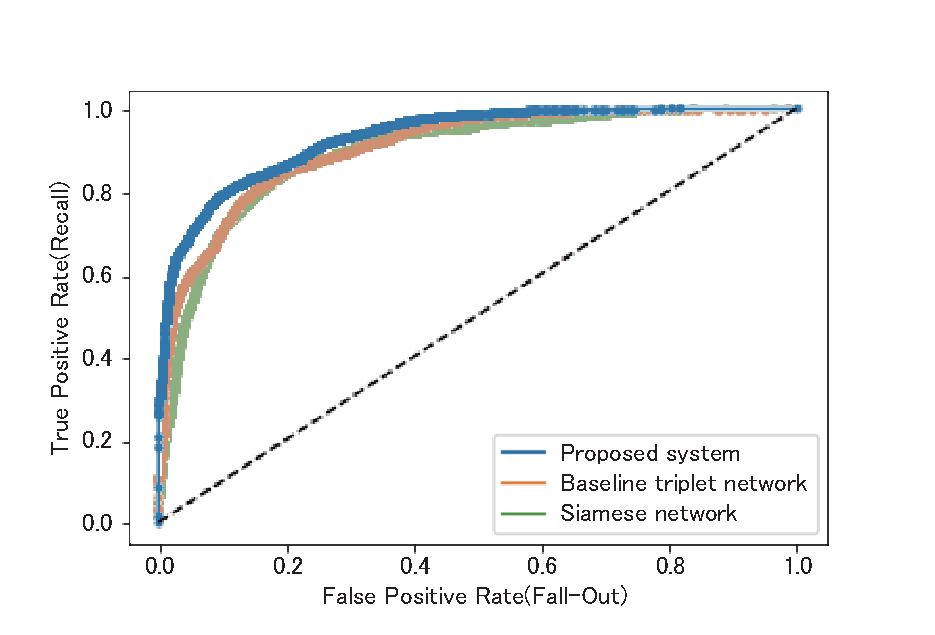
\includegraphics[height=6.4cm]{fig_roc_v11.eps}}
    \subfigure[][Normalized training loss curve]{
        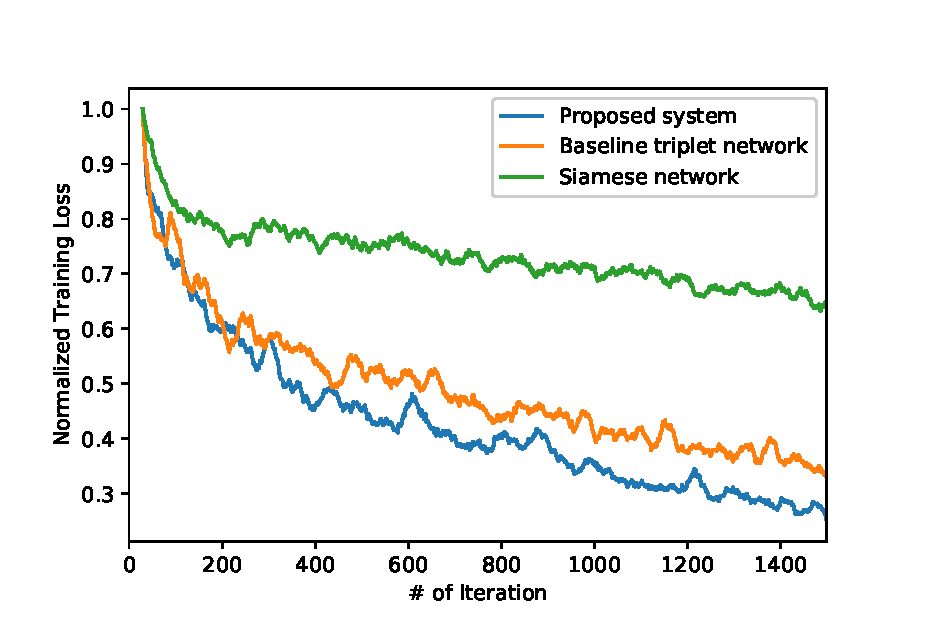
\includegraphics[height=6.4cm]{normalized_loss_curve_ma30_v2.eps}}
    \caption{(a) shows the Receiver Operating Characteristic(ROC) Curve and 
    (b) shows the normalized training loss curve of the deep learning based methods. }
    \label{fig2}
    \end{center}
 \end{figure}

\section{Conclusion}
In this paper, we proposed a system for identity verification based on the handwritten signature signals captured by the Wi-Fi CSI signals. 
The kernel and the range space learning was initially adopted for refining the triplet inputs for fast loss convergence by mining the distinctive inputs from the training Wi-Fi signature signals. 
Subsequently, the triplet network utilizing the ConvNet structure was trained with the mined triplet inputs based on L-2 distance comparison. 
Our experiments on an in-house Wi-Fi handwritten signature signal dataset showed encouraging verification accuracy with faster training loss convergence compared with the baseline triplet network and the Siamese network.
%
% ---- Bibliography ----
%
% BibTeX users should specify bibliography style 'splncs04'.
% References will then be sorted and formatted in the correct style.
%
%\bibliographystyle{splncs04}
%\bibliography{mybibliography}
%


%\begin{thebibliography}{8}
\clearpage
\bibliographystyle{splncs04}
\bibliography{bib_acpr}

%\end{thebibliography}

\end{document}